\documentclass[12pt]{article}
\usepackage{amsmath, amssymb, booktabs, threeparttable, graphicx, pdflscape}
\usepackage[margin=1in]{geometry}
\usepackage{apacite}
\usepackage{setspace}
\doublespacing
\setlength\parindent{1.5em}

\title{Diagnostic Inflation Expectations in China:\\ The Role of Economics Policy Uncertainty and Geopolitical Risk}
\author{Jingle Fu}
\date{\today}

\begin{document}
\maketitle

\begin{abstract}
    Household inflation expectations often respond disproportionately to salient news, generating systematic forecast errors. This paper tests whether Chinese households exhibit a \emph{diagnostic} pattern—expectation revisions that subsequently predict forecast errors of opposite sign—using the PBoC Urban Depositors Survey. We quantify qualitative responses into a numeric expectation measure via the Carlson–Parkin method and evaluate diagnostic bias through a HAC-robust OLS baseline and a Bayesian time-varying-parameter state-space model (TVP-SSM). The OLS analysis suggests a negative relationship between forecast revisions and subsequent forecast errors, though imprecisely estimated in the small sample. The Bayesian TVP-SSM reveals that this diagnostic coefficient is predominantly negative across time, with posterior mean approximately -0.52, becoming particularly pronounced around major macro events. While uncertainty measures (EPU/GPR) are correlated with these episodes, their incremental explanatory power in linear drift specifications is limited, suggesting mechanisms may be nonlinear or event-driven. Finally, we use a sign-restricted Bayesian VAR to characterize a set-identified class of shocks consistent with the diagnostic overreaction-correction pattern, interpreting the results as dynamic evidence consistent with behavioral theory rather than a uniquely identified structural mechanism.
\end{abstract}

\section{Introduction}
The formation of inflation expectations is a cornerstone of modern macroeconomic theory and policy. While the rational expectations hypothesis remains a canonical modeling device, a wealth of empirical evidence from household and professional surveys documents persistent and systematic deviations from full-information rationality. Understanding the nature of these deviations is particularly critical for emerging economies like China, where monetary policy frameworks are evolving and household sentiment can significantly influence economic dynamics.

Chinese household inflation expectations, as recorded in the People's Bank of China (PBoC) quarterly survey, exhibit puzzling features: systematic forecast errors, volatility patterns, and episodes of sharp overreaction to transitory price shocks. These patterns invite an examination through the lens of behavioral economics. This paper investigates whether Chinese household expectations are consistent with the theory of \emph{diagnostic expectations} \cite{Bordalo2018}. This framework, which formalizes the representativeness heuristic, posits that agents overweight salient or surprising information, leading to predictable forecast errors characterized by overreaction and subsequent correction.

China's recent economic history provides a compelling setting for this inquiry. The period from 2013 to 2025 witnessed repeated surges in economic policy uncertainty (EPU), related to domestic financial reforms and shifting growth paradigms, and spikes in geopolitical risk (GPR), most notably from U.S.-China trade tensions and global conflicts. These factors likely influence how households process information about future prices. We ask: Do Chinese households exhibit diagnostic biases in forming inflation expectations? And are these biases amplified during periods of high uncertainty or geopolitical stress?

Answering these questions requires careful empirical strategies that address two key challenges. First, one must align the quantitative measure of expected inflation derived from qualitative surveys with an appropriate measure of realized inflation, ensuring a valid test of forecast accuracy. Second, identifying a structural shock that embodies diagnostic overreaction requires moving beyond simple correlations to isolate disturbances that have the distinct dynamic signature predicted by the theory.

Our analysis employs two complementary Bayesian approaches to meet these challenges. First, we estimate a time-varying parameter state-space model (TVP-SSM) that directly relates forecast errors to prior forecast revisions. This model allows the key diagnostic parameter $\beta_t$ to evolve over time, and we examine its association with EPU and GPR. Second, we estimate a Bayesian vector autoregression (BVAR) with sign restrictions to characterize a class of shocks consistent with the diagnostic pattern. Our identification strategy is explicitly derived from the theoretical mechanism: we search for shocks that generate an immediate rise in inflation expectations, a weaker contemporaneous response in actual inflation, and a pattern where future inflation realizations lag behind contemporaneous expectations, thereby producing negative forecast errors. To sharpen the identification, we impose additional restrictions informed by the narrative of a positive news-driven overreaction, such as a rise in industrial output.

Our findings present a coherent picture. The TVP-SSM reveals that the relationship between forecast revisions and subsequent errors is consistently negative, with a posterior mean for $\beta_t$ of approximately -0.52. This diagnostic bias is not constant; it becomes markedly stronger during acute stress episodes like the 2015-16 financial market turbulence, the 2018-19 trade war escalation, and the initial COVID-19 shock in 2020. The BVAR analysis corroborates this by isolating a shock that precisely generates the predicted overreaction-correction dynamic. This shock causes a large, immediate jump in expected inflation but only a muted increase in actual inflation, leading to a sequence of negative forecast errors that persist for several quarters. Notably, this shock is associated with rising output and falling uncertainty, consistent with an overreaction to positive growth news. In terms of economic significance, this diagnostic news shock explains about 25-30\% of the short-term variance in inflation expectations but less than 10\% of the variance in actual inflation, indicating that while expectation swings are substantial, their self-fulfilling potential appears limited under prevailing policy and market structures.

This paper contributes to several literatures. First, it provides one of the first comprehensive tests of the diagnostic expectations hypothesis in a major emerging economy, extending a framework developed primarily in advanced-economy contexts to a setting with distinct institutional and informational features. Second, methodologically, it demonstrates how sign restrictions grounded in behavioral theory can be used to identify structurally meaningful expectation shocks, offering a template for future research. Third, it delivers new insights into the dynamics of Chinese inflation expectations, highlighting the role of behavioral biases that may complicate the transmission of monetary policy. For policymakers, our results underscore the importance of clear, consistent communication, especially during periods of high uncertainty, to mitigate salience-driven overreactions that could distort household planning and economic outcomes.

The remainder of the paper proceeds as follows. Section \ref{sec:lit} reviews the relevant theoretical and empirical literature. Section \ref{sec:data} describes our data sources, the construction of key variables—paying special attention to the alignment of forecast horizons—and presents descriptive statistics. Section \ref{sec:methods} details the TVP-SSM and sign-restricted BVAR methodologies. Sections \ref{sec:results_ssm} and \ref{sec:results_bvar} present the core empirical results. Section \ref{sec:discussion} discusses the implications of our findings, considers alternative interpretations, and explores limitations. Section \ref{sec:conclusion} concludes.

\section{Literature and Theoretical Framework}\label{sec:lit}
\subsection{Expectation Formation: From Rationality to Diagnosticity}
The rational expectations hypothesis (REH), a bedrock of modern macroeconomics, posits that agents form forecasts using all available information and a (subjective) understanding of the economy's true structure, resulting in errors that are unpredictable \cite{Muth1961, Lucas1972}. This assumption imbues macroeconomic models with internal consistency and sharp policy implications. However, persistent empirical puzzles—such as the excess volatility of asset prices, the slow adjustment of professional forecasts, and systematic biases in household surveys—have prompted economists to incorporate richer psychological foundations into models of belief formation \cite{Shiller2000, Akerlof2009}.

Diagnostic expectations \cite{Bordalo2018} offer a parsimonious and powerful behavioral alternative. Rooted in Kahneman and Tversky's representativeness heuristic, the theory proposes that when agents evaluate uncertain prospects, they overweight future states that are ``representative'' of, or similar to, recently observed signals. In a dynamic updating context, this leads to an overreaction to news. Formally, diagnostic expectations can be expressed as a distortion of standard Bayesian updating:
\[
    \mu_t^{\text{diag}} = \mu_t^{\text{Bayes}} + \theta \cdot (S_t - \mathbb{E}_{t-1}[S_t]),
\]
where $\mu_t$ denotes the belief, $S_t$ is a noisy signal, and $\theta > 0$ is a parameter capturing the degree of overreaction. When $\theta=0$, beliefs are rational (Bayesian); when $\theta>0$, agents over-extrapolate, assigning excessive weight to the surprise component of the signal.

This mechanism yields a clear empirical fingerprint: a negative correlation between forecast revisions and subsequent forecast errors. A positive revision in expectations (driven by a surprisingly high signal) should, on average, be followed by a negative forecast error as reality reverts toward its fundamental path. This prediction stands in contrast to models of informational rigidities like sticky information \cite{Mankiw2002} or rational inattention \cite{Sims2003}, which typically generate \emph{underreaction} and positive serial correlation in forecast errors.

\subsection{Uncertainty, Geopolitical Risk, and Attention}
The diagnostic expectations framework naturally interacts with the broader information environment. Economic policy uncertainty (EPU), reflecting ambiguity about future fiscal, regulatory, or monetary policy, can influence how agents process signals \cite{Baker2016}. High uncertainty may lower the signal-to-noise ratio, which in a rational model should lead to more cautious updating. However, from a behavioral perspective, heightened anxiety and media focus during uncertain times could instead amplify the salience of extreme news, potentially exacerbating diagnostic overreactions. The net effect is an empirical question.

Geopolitical risk (GPR), encompassing threats of war, terrorism, and diplomatic conflict, represents a more visceral and narrative-driven class of shocks \cite{Caldara2022}. For an open economy like China, GPR shocks directly affect perceived inflation risks through channels such as commodity price spikes (e.g., oil, food), supply chain disruptions, and exchange rate pressure. The sudden, dramatic nature of geopolitical events may make them particularly potent triggers of the representativeness heuristic, leading households to over-infer a new regime of higher inflation from a temporary shock.

\subsection{Empirical Identification and the Chinese Context}
Testing for diagnostic expectations requires confronting two main tasks: establishing the reduced-form correlation pattern and, more ambitiously, identifying structural shocks that embody the theorized mechanism.

The reduced-form test is straightforward: in a regression of the forecast error $FE_t = \pi_{t+1} - \mu_t$ on the prior forecast revision $FR_t = \mu_t - \mu_{t-1}$, a significantly negative coefficient $\beta$ is consistent with diagnostic overreaction. We acknowledge that since $FE_t$ and $FR_t$ both contain $\mu_t$, measurement error in expectations could mechanically induce some negative correlation (``coupling bias''). However, we use this regression primarily as a preliminary diagnostic signature before moving to the state-space and VAR analysis.

Structural identification is more challenging. The goal is to isolate a shock that causes expectations to move excessively relative to the eventual inflation outcome. Simply requiring that a shock raises $\mu_t$ more than $\pi_t$ is insufficient, as many shocks could produce this short-run pattern. The theoretical essence of a diagnostic shock is that it represents an \emph{overreaction to fundamental news}. Therefore, a more compelling identification would seek a shock that: (1) raises expectations sharply; (2) has a muted initial impact on actual inflation; and (3) is associated with movements in other variables (like output) that are consistent with a response to news about future economic conditions. We implement this approach using sign restrictions in a BVAR.

China presents a distinctive laboratory. Households may rely more on observable price changes in frequently purchased goods (like food, particularly pork) and on state-media narratives than on central bank communications or complex macroeconomic models. The well-known ``Pork Cycle'' in China drives significant volatility in CPI, often dominating household perceptions of living costs regardless of core inflation trends. This context may make expectations especially susceptible to salience-driven biases, providing a strong test for the diagnostic framework.

\section{Data and Variable Construction}\label{sec:data}
\subsection{Survey Data and Sample Coverage}
Our primary data source is the Urban Depositors Survey conducted quarterly by the People's Bank of China (PBoC). This survey covers 50 major cities and samples approximately 20,000 urban households each quarter, collecting qualitative perceptions and expectations on a range of economic indicators including income, employment, housing prices, and overall prices. The key question for our purposes is: ``How do you expect the price level next quarter will compare to this quarter?'' Respondents choose from ``rise,'' ``basically unchanged,'' ``fall,'' or ``uncertain.'' The PBoC publishes a composite Future Price Expectations Index based on these responses, which ranges theoretically from 0 to 200, with 100 indicating neutral expectations.

Our full sample initially spans 2011Q1 to 2025Q3 for the expectations index. However, not all quarters have the detailed breakdown of responses needed for quantification. After data cleaning, we can compute quantitative expectations for 48 quarters, covering 2013Q1 to 2025Q3. The effective estimation sample for the TVP-SSM and BVAR, after accounting for the need for lagged expectations and forward inflation, runs from 2013Q4 through 2025Q2, yielding 43 quarterly observations.

It is worth noting that our sample period covers a variety of economic conditions in China: the ``new normal'' of slower growth around 2014-2015, the supply-side structural reforms of 2016-2018, the onset of U.S.-China trade tensions in 2018-2019, the COVID-19 shock in 2020-2021, and the post-pandemic recovery with global inflation pressures in 2022-2023. Thus, our sample encompasses both disinflationary and inflationary expectation environments, lending representativeness to our findings.

\subsection{Quantifying Inflation Expectations: The Carlson-Parkin Method}\label{sec:cp_method}
The qualitative survey responses must be converted into a numeric expected inflation rate. We apply the classical \cite{Carlson1975} probabilistic method. The approach assumes each respondent has in mind a subjective probability distribution for next-period inflation, with mean $\mu_t$ and standard deviation $\sigma_t$. The respondent answers ``rise'' if they believe inflation will exceed some threshold $U$, ``fall'' if it will be below some threshold $L$, and ``unchanged'' if in between. Under Carlson-Parkin, one typically assumes a symmetric indifference band around zero, that is, $U = -L = \delta$, meaning if expected inflation change is within $[-\delta, +\delta]$, the respondent views it as ``about the same.''

Specifically, let $p^{up}_t$ be the fraction of respondents expecting prices to increase, and $p^{down}_t$ the fraction expecting a decrease, after excluding the ``uncertain'' responses. Assuming $\pi_{t+1} \sim N(\mu_t, \sigma_t^2)$, we have:
\[
    p^{down}_t = \Pr(\pi_{t+1} < L) = \Phi\!\Big(\frac{L - \mu_t}{\sigma_t}\Big), \qquad
    p^{up}_t = \Pr(\pi_{t+1} > U) = 1 - \Phi\!\Big(\frac{U - \mu_t}{\sigma_t}\Big).
\]
With the symmetric indifference interval assumption ($U=-L=\delta$), these simplify to:
\[
    p^{down}_t = \Phi\!\Big(\frac{-\delta - \mu_t}{\sigma_t}\Big), \qquad
    p^{up}_t = 1 - \Phi\!\Big(\frac{\delta - \mu_t}{\sigma_t}\Big).
\]
Define the standardized normal quantiles $z_d \equiv \Phi^{-1}(p^{down}_t)$ and $z_u \equiv \Phi^{-1}(1 - p^{up}_t)$, which represent the $z$-scores corresponding to the observed probabilities. Then the system can be written as:
\[
    z_d = \frac{-\delta - \mu_t}{\sigma_t}, \qquad z_u = \frac{\delta - \mu_t}{\sigma_t}.
\]
Solving for $\mu_t$ and $\sigma_t$ yields:
\[
    \sigma_t = \frac{2\delta}{\,z_u - z_d\,}, \qquad
    \mu_t = -\delta - \sigma_t \cdot z_d = \delta - \sigma_t \cdot z_u~.
\]

In practice, a calibration for $\delta$ is needed. The literature often either assumes a fixed indifference interval or estimates it from historical data. We follow common practice by choosing $\delta = 0.5$ percentage points, reflecting that respondents view price moves within $\pm 0.5$ percentage points as essentially ``unchanged.'' This choice is in line with other survey quantifications and provides a reasonable fit to historical revisions. The thresholds are symmetric around zero: respondents answering ``rise'' expect inflation above +0.5pp, those answering ``fall'' expect below -0.5pp, and ``unchanged'' corresponds to the interval $[-0.5, +0.5]$. Our results are not sensitive to moderate variations in $\delta$—sensitivity analysis with $\delta \in \{0.3, 0.4, 0.5, 0.6, 0.7\}$ yields qualitatively similar patterns of diagnostic bias.

One additional complication is the ``uncertain'' responses. We handle these by first removing the ``uncertain'' percentage from the total and renormalizing $p^{up}_t$, $p^{down}_t$, $p^{same}_t$ to sum to 1. Effectively, we assume respondents who answered ``uncertain'' have no systematic bias and their exclusion does not affect the aggregate probabilities of the others. During our sample, the ``uncertain'' option was chosen by about 15 percent of respondents on average, spiking above 25 percent in extreme events such as 2020Q1 at the onset of COVID-19. The high share of ``uncertain'' itself reflects public confusion during extreme uncertainty. In those periods, the remaining respondents might disproportionately include those with strong directional views, so our $\mu_t$ could be based on a more polarized subset. However, since the Carlson-Parkin method presumes a representative agent interpretation of the proportions, we proceed with the standard adjustment.

\subsection{Aligning Expectations with Realizations: The Horizon Issue}\label{sec:horizon}
A critical issue in testing forecast accuracy is aligning the forecast horizon. The PBoC survey asks about price changes over the **next quarter**. Therefore, to construct a commensurate measure of realized inflation, we construct the **Quarter-on-Quarter (QoQ) Annualized CPI inflation rate** for quarter $t+1$. We derive this from the seasonally adjusted CPI index (reconstructed from monthly data). Specifically, $\pi_{t+1}^{QoQ, ann} = [ (P_{t+1}/P_{t})^4 - 1 ] \times 100$, where $P_t$ is the price level at the end of quarter $t$. This measure aligns with the quarterly forecast horizon while being scaled to annual terms (percentage points) to match the standard reporting convention.

The forecast error is defined as $FE_t = \pi_{t+1}^{QoQ, ann} - \mu_t$, and the forecast revision as $FR_t = \mu_t - \mu_{t-1}$. Our final estimation sample runs from 2013Q4 to 2025Q2, yielding 43 quarterly observations.

\subsection{Units and Scaling Check}
It is important to clarify the units of our quantified variables. As shown in Table \ref{tab:desc_stats}, quantified expectations $\mu_t$ have a mean of approximately 0.45 percentage points (annualized), while realized QoQ annualized inflation $\pi_t$ has a mean of approximately 1.75 percentage points, both measured in the same units but with different central tendencies. This difference reflects the sample-period average forecast error. The fixed indifference parameter $\delta=0.5$ in the Carlson-Parkin method acts as a threshold for ``unchanged'' responses.

\subsection{Uncertainty, Risk, and Control Variables}
We incorporate the China Economic Policy Uncertainty Index \cite{Baker2016} and the Global Geopolitical Risk Index \cite{Caldara2022}, averaging their monthly values to quarterly frequency. The China EPU index is constructed via news article counts in the South China Morning Post. In our sample the EPU index has several notable spikes: it jumped during the 2015 stock market crash and RMB exchange rate reform, reached a peak during the initial U.S.-China trade dispute in 2018, and spiked again in early 2020 during COVID-19. The global GPR index captures worldwide geopolitical risk events. It spikes around events like the 2014 Crimea crisis, the 2017 North Korea missile crisis, and reaches its highest value in early 2022 with the Russia-Ukraine war.

To account for other potential determinants of forecast errors, we include control variables in some specifications: industrial value added growth (a proxy for the business cycle), broad money (M2) growth (controlling for monetary conditions and liquidity), producer price index (PPI) inflation (upstream price pressure), and food CPI inflation. Food prices—especially pork in China—often drive short-term CPI swings and consumer sentiment, representing a particularly salient channel through which households form expectations. All data are sourced from the PBoC, the National Bureau of Statistics of China, and the cited index creators.

\subsection{Descriptive Evidence}
Table \ref{tab:desc_stats} and Table \ref{tab:fe_fr} present summary statistics. Several features stand out. First, the forecast error statistics reveal that the mean forecast error $FE_t$ is positive (+1.13 percentage points), indicating that, on average, actual inflation turned out higher than households expected. This suggests a systematic under-prediction bias in our sample period. This finding differs from some international evidence showing over-estimation, and may reflect China's specific context: households anchoring expectations to the low-inflation ``new normal'' period of the mid-2010s, subsequently surprised by food price shocks (pork cycle) and global inflation spillovers post-2020. Second, the uncertainty and risk indices exhibit large variation (EPU in particular varies by a factor of six from trough to peak), mirroring the turbulent economic and geopolitical environment of the 2013-2025 period.

Most importantly, there is a negative correlation between $FE_t$ and $FR_t$ ($r=-0.19$, as detailed in Table \ref{tab:corr_matrix}), providing initial evidence that when expectations go up, subsequent errors tend to be negative, and vice versa. A basic OLS regression (Table \ref{tab:ols_baseline}) yields a negative coefficient on forecast revisions, which is marginally significant at the 10\% level in specifications including control variables. While the relationship is imprecisely estimated given the limited sample size (N=43), the sign is consistent with diagnostic overreaction. This regression, albeit simple, foreshadows our main results: a negative coefficient on forecast revisions is exactly what diagnostic expectations theory predicts. We turn to Bayesian methods for more precise inference.

\begin{table}[!htbp]
    \centering
    \small
    \caption{Descriptive Statistics of Key Variables (Quarterly)}
    \label{tab:desc_stats}
    \begin{threeparttable}
        \begin{tabular}{@{}lllllllll@{}}
            \toprule
            variable               & count  & mean    & std     & min    & 25\%    & median  & 75\%    & max     \\
            \midrule
            infl\_exp\_index       & 58.000 & 62.862  & 4.294   & 56.100 & 59.650  & 61.800  & 64.375  & 74.800  \\
            $\mu_{cp} $            & 48.000 & 0.452   & 0.551   & -1.287 & 0.120   & 0.411   & 0.704   & 1.736   \\
            % CPI\_YoY               & 58.000 & 100.141 & 0.269   & 99.426 & 99.957  & 100.160 & 100.333 & 100.668 \\
            CPI\_QoQ\_Ann          & 58.000 & 1.746   & 3.266   & -6.679 & -0.514  & 1.938   & 4.049   & 8.314   \\
            Food\_CPI\_YoY\_qavg   & 58.000 & 3.498   & 5.276   & -5.148 & -0.342  & 2.665   & 5.458   & 20.299  \\
            epu\_qavg              & 58.000 & 225.325 & 112.921 & 75.909 & 125.531 & 222.375 & 306.892 & 499.249 \\
            gpr\_qavg              & 58.000 & 105.028 & 29.137  & 69.691 & 87.027  & 95.891  & 118.628 & 224.596 \\
            Ind\_Value\_Added\_YoY & 58.000 & 5.867   & 3.152   & -0.367 & 3.958   & 5.883   & 7.017   & 13.933  \\
            M2\_YoY                & 58.000 & 10.893  & 2.536   & 6.480  & 8.542   & 10.950  & 13.033  & 16.510  \\
            \bottomrule
        \end{tabular}
        \begin{tablenotes}[flushleft]
            \footnotesize
            \item Mean/Std calculated using available sample. See data appendix for variable definitions.
        \end{tablenotes}
    \end{threeparttable}
\end{table}


\begin{table}[!htbp]
\centering
\small
\caption{Forecast Error and Revision Statistics}
\label{tab:fe_fr}
\begin{threeparttable}
    \begin{tabular}{@{}lrrrrrrrr@{}}
        \toprule
        Variable & $N$ & Mean & Std.\ Dev. & Min & P25 & Median & P75 & Max \\
        \midrule
        Forecast Error ($FE$) & 43.000 & 1.130 & 3.171 & -7.004 & -0.670 & 1.453 & 3.110 & 7.611 \\
        Forecast Revision ($FR$) & 43.000 & -0.051 & 0.507 & -1.612 & -0.306 & -0.042 & 0.319 & 0.916 \\
        \addlinespace
        Corr($FE$, $FR$) & 43.000 & -0.192 &  &  &  &  &  &  \\
        \bottomrule
    \end{tabular}
    \begin{tablenotes}[flushleft]
        \footnotesize
        \item \textit{Notes:} $FE_t = CPI_{t+1} - \mu_t$ (forecast error) and $FR_t = \mu_t - \mu_{t-1}$ (forecast revision).
        \item A negative Corr($FE$, $FR$) is consistent with diagnostic expectations.
    \end{tablenotes}
\end{threeparttable}
\end{table}


\begin{table}[htbp]
\centering
\begin{threeparttable}
\caption{Baseline Forecast-Error Regressions}
\label{tab:ols_baseline}
{\small
\begin{tabular}{lcccc}
\toprule
 & \multicolumn{4}{c}{Dependent variable: Forecast error$_{t+1}$} \\
\cmidrule(lr){2-5}
 & (1) & (2) & (3) & (4) \\
 & Bivariate & +Macro & +Uncertainty & Alt.\ Revision \\
\midrule
$\hat{\beta}$ (revision) & $-1.662^{*}$ & $-2.237^{*}$ & $-2.125$ & $0.535^{***}$ \\
 & (0.957) & (1.114) & (1.256) & (0.080) \\
\addlinespace
Observations & 32 & 32 & 32 & 36 \\
$R^2$ & 0.048 & 0.157 & 0.186 & 0.281 \\
\addlinespace
Province FE & $\times$ & $\times$ & $\times$ & $\times$ \\
Wave FE & $\times$ & $\times$ & $\times$ & $\times$ \\
Demographics & $\times$ & $\times$ & $\times$ & $\times$ \\
Macro controls & $\times$ & $\checkmark$ & $\checkmark$ & $\checkmark$ \\
Uncertainty controls & $\times$ & $\times$ & $\checkmark$ & $\times$ \\
\bottomrule
\end{tabular}
}
\begin{tablenotes}[flushleft]
\footnotesize
\item \textit{Notes:} Dependent variable is next-quarter forecast error using Carlson--Parkin expectations. Standard errors (in parentheses) are Newey--West HAC with 4 lags (time-series setting; no cross-sectional clustering). $^{*}p<0.10$; $^{**}p<0.05$; $^{***}p<0.01$.
\end{tablenotes}
\end{threeparttable}
\end{table}


Table \ref{tab:corr_matrix} presents the pairwise correlations among our key variables. The quantified expectation $\mu_t$ correlates positively with actual CPI inflation, but this correlation is far from perfect, confirming that expectations contain substantial variation independent of actual outcomes. As shown in the table, the negative correlation between $FE_t$ and forecast revision $FR_t$ provides the key diagnostic signature. EPU shows a moderately negative correlation with $\mu_t$, possibly because EPU surges often coincide with deflation fears or demand collapse scenarios. GPR's correlations are generally smaller in magnitude, suggesting geopolitical risk has more idiosyncratic effects not strongly captured by linear associations.

\begin{table}[!htbp]
    \centering
    \caption{Correlation Matrix of Key Variables (Lower Triangle)}
    \label{tab:corr_matrix}
    \begin{tabular}{@{}llllllllll@{}}
        \toprule
        Variable   & $\mu_{CP}$ & CPI    & FE     & FR     & Food   & EPU    & GPR    & M2     & PPI   \\
        \midrule
        $\mu_{CP}$ & 1.000      &        &        &        &        &        &        &        &       \\
        CPI        & 0.539      & 1.000  &        &        &        &        &        &        &       \\
        FE         & -0.905     & -0.651 & 1.000  &        &        &        &        &        &       \\
        FR         & 0.453      & 0.653  & -0.451 & 1.000  &        &        &        &        &       \\
        Food       & 0.139      & 0.192  & -0.164 & -0.116 & 1.000  &        &        &        &       \\
        EPU        & -0.458     & -0.036 & 0.449  & 0.011  & 0.185  & 1.000  &        &        &       \\
        GPR        & -0.169     & -0.034 & 0.105  & 0.040  & -0.421 & 0.097  & 1.000  &        &       \\
        M2         & 0.343      & -0.040 & -0.312 & -0.077 & 0.185  & -0.456 & -0.156 & 1.000  &       \\
        PPI        & -0.063     & 0.092  & 0.114  & 0.060  & -0.334 & 0.140  & 0.015  & -0.345 & 1.000 \\
        \bottomrule
    \end{tabular}
    \begin{flushleft}\footnotesize
        Only the lower-triangle of the matrix is shown to save space.\\
        Diagonal entries equal 1 (omitted for brevity).\\
        Calculated on the sample with no missing values for all variables.
    \end{flushleft}
\end{table}


Table \ref{tab:subperiod} examines whether diagnostic expectations behavior differs across distinct macroeconomic regimes by splitting the sample into pre-2018 and 2018-onward subperiods. The year 2018 marks an important structural break when U.S.-China trade tensions escalated sharply. Comparing the two subperiods, we observe striking differences. Quantified expectations $\mu_t$ were notably higher in the 2011-2017 period compared to 2018-2025, reflecting that Chinese inflation has been generally lower and more stable in recent years. However, the mean forecast error ($FE_t=\pi^{QoQ,ann}_{t+1}-\mu_t$) remains positive in both subperiods (0.90 in 2011-2017, 0.98 in 2018-2025), indicating persistent under-prediction on average. The subperiod differences are more pronounced in dispersion and tail realizations rather than in the mean, suggesting that regime changes may affect the volatility of errors and revisions more than their unconditional direction. Crucially, uncertainty measures jumped dramatically in the post-2018 period, with EPU nearly tripling and GPR also rising substantially. These increases underscore that the post-2018 period was characterized by unprecedented policy and geopolitical uncertainty. This sets the stage for understanding why a time-varying approach is necessary: the relationship between expectation updates and subsequent errors adapts to the macroeconomic environment.

\begin{table}[!htbp]
    \centering
    \small
    \caption{Sub-period Statistics: Pre vs Post 2018}
    \label{tab:subperiod}
    \begin{threeparttable}
        \begin{tabular}{@{}lllllll@{}}
            \toprule
            Period                   & Variable      & N      & Mean    & Std    & Min     & Max     \\
            \midrule
            2013-2017 ($\mu$ sample) & mu\_cp        & 18.000 & 0.793   & 0.491  & 0.171   & 1.736   \\
            2013-2017 ($\mu$ sample) & CPI\_QoQ\_Ann & 18.000 & 1.892   & 3.007  & -4.322  & 6.825   \\
            2013-2017 ($\mu$ sample) & FE            & 18.000 & 0.896   & 3.044  & -5.749  & 6.055   \\
            2013-2017 ($\mu$ sample) & FR            & 15.000 & -0.075  & 0.418  & -0.902  & 0.650   \\
            2013-2017 ($\mu$ sample) & epu\_qavg     & 18.000 & 128.780 & 50.384 & 75.909  & 277.163 \\
            2013-2017 ($\mu$ sample) & gpr\_qavg     & 18.000 & 99.150  & 17.208 & 73.702  & 135.585 \\
            2018-2025 ($\mu$ sample) & mu\_cp        & 30.000 & 0.247   & 0.485  & -1.287  & 1.270   \\
            2018-2025 ($\mu$ sample) & CPI\_QoQ\_Ann & 30.000 & 1.443   & 3.292  & -6.679  & 8.314   \\
            2018-2025 ($\mu$ sample) & FE            & 29.000 & 0.980   & 3.337  & -7.004  & 7.611   \\
            2018-2025 ($\mu$ sample) & FR            & 29.000 & -0.010  & 0.566  & -1.612  & 0.916   \\
            2018-2025 ($\mu$ sample) & epu\_qavg     & 30.000 & 305.227 & 71.802 & 165.772 & 453.896 \\
            2018-2025 ($\mu$ sample) & gpr\_qavg     & 30.000 & 114.319 & 35.227 & 69.691  & 224.596 \\
            \bottomrule
        \end{tabular}
        \begin{tablenotes}[flushleft]
            \footnotesize
            \item Subperiods based on quarters with non-missing $\mu_{cp} $ (2013Q1-2025Q3).
            \item 2018 marks the escalation of US-China trade tensions.
            \item EPU and GPR means rose in the post-2018 period.
        \end{tablenotes}
    \end{threeparttable}
\end{table}


\section{Empirical Methodology}\label{sec:methods}
\subsection{A Time-Varying Parameter State-Space Model (TVP-SSM)}
To model the evolving relationship between forecast errors and revisions, we specify a state-space model. The measurement equation is:
\begin{equation}\label{eq:measurement}
    FE_t = \alpha + \beta_t FR_t + \gamma' Z_t + \varepsilon_t, \qquad \varepsilon_t \sim \mathcal{N}(0, R),
\end{equation}
where $Z_t$ is a vector of control variables (food inflation, M2 growth, PPI inflation). The time-varying coefficient $\beta_t$ captures the diagnostic bias. A negative $\beta_t$ indicates that a positive forecast revision predicts a negative future error.

The state equation governs the evolution of $\beta_t$:
\begin{equation}\label{eq:state}
    \beta_t = \beta_{t-1} + d_{\text{EPU}} \Delta \text{EPU}_t + d_{\text{GPR}} \Delta \text{GPR}_t + u_t, \qquad u_t \sim \mathcal{N}(0, Q).
\end{equation}
This allows the bias to follow a random walk with a drift component that depends on changes in the uncertainty indices ($\Delta EPU_t, \Delta GPR_t$). The coefficients $d_{\text{EPU}}$ and $d_{\text{GPR}}$ test whether rising uncertainty linearly amplifies the diagnostic bias.

We estimate the model using Bayesian methods. Priors are chosen to be relatively diffuse but proper: $\beta_0 \sim \mathcal{N}(-0.5, 0.5^2)$, $d_{\text{EPU}}, d_{\text{GPR}} \sim \mathcal{N}(0, 0.2^2)$, and $R, Q \sim \mathcal{IG}(3, 0.001)$. The Gibbs sampler iterates between drawing the latent state path $\{\beta_t\}$ via the forward-filtering backward-sampling algorithm and drawing the static parameters conditional on the states.

\subsection{Identifying a Diagnostic News Shock with Sign Restrictions}
To move beyond correlations and explore the dynamic macroeconomic effects of a diagnostic bias, we estimate a Bayesian VAR and identify a structural shock using sign restrictions \cite{Uhlig2005}. The VAR includes five variables: $y_t = (\mu_t, \pi_t, g_t, EPU_t, GPR_t)'$, where $g_t$ is industrial production growth. We include two lags and use a Minnesota prior.

Let the reduced-form VAR be $y_t = c + A_1 y_{t-1} + A_2 y_{t-2} + \epsilon_t$, with $\epsilon_t \sim \mathcal{N}(0, \Sigma)$. A structural shock is identified via an orthogonalization $\epsilon_t = B \eta_t$, where $\eta_t \sim \mathcal{N}(0, I)$ and $B$ satisfies $BB' = \Sigma$. Any $B = P Q$ is valid, where $P$ is the Cholesky factor of $\Sigma$ and $Q$ is an orthonormal matrix.

We search for a column of $B$ (a shock) whose impulse responses satisfy a set of sign restrictions designed to capture a ``diagnostic news shock.'' The key theoretical insight is that we seek to identify a disturbance that generates overreaction in expectations to news about future economic conditions, rather than simply any shock that raises expectations. Simply requiring that a shock raises $\mu_t$ more than $\pi_t$ would be insufficient, as many shocks could produce this short-run pattern. The theoretical essence of a diagnostic shock is that it represents an overreaction to fundamental news.

Therefore, our identification strategy imposes restrictions that distinguish a diagnostic shock from alternative interpretations such as a pure noise shock or a conventional demand shock. Specifically, our baseline restrictions are:
\begin{itemize}
    \item \textbf{On impact ($h=0$):} $IRF_{\mu}(0) > 0$, $IRF_{\pi}(0) > 0$, and $IRF_{g}(0) > 0$.
    \item \textbf{For horizons $h = 0, 1, 2$:} $IRF_{\pi}(h+1) - IRF_{\mu}(h) < 0$.
\end{itemize}

The first set requires the shock to initially raise inflation expectations, actual inflation, and output—a pattern suggestive of a positive demand or growth news shock rather than a pure sentiment noise shock (which would not affect output). The second set imposes the diagnostic signature: expected inflation in any period exceeds the realized inflation in the next period, creating negative forecast errors. We leave the responses of $EPU_t$ and $GPR_t$ unrestricted, allowing the data to reveal whether such shocks occur when uncertainty resolves or rises.

This identification strategy goes beyond circular definition in three ways. First, by requiring a positive output response, we ensure the shock represents genuine economic news (an expansion) rather than spurious sentiment. Second, we impose the forecast error pattern for multiple horizons, not just on impact, ensuring persistence of the diagnostic mechanism. Third, the extremely high acceptance rate (over 99.95 percent) indicates that the restrictions define a relatively permissive identified set. We therefore interpret the resulting IRFs as set-identified dynamic patterns consistent with the diagnostic signature, rather than as evidence of a uniquely pinned-down structural shock. We also conduct robustness checks where we relax the output restriction or impose it only on impact, yielding quantitatively similar results.
\begin{table}[!htbp]
    \centering
    \caption{BVAR sign-restriction acceptance}
    \label{tab:bvar_accept}
    \begin{tabular}{rrrrr}
        \toprule
        accepted\_draws & posterior\_draws & rotations\_per\_draw & total\_rotations & accept\_rate\_per\_posterior\_draw \\
        \midrule
        1999            & 2000             & 200                  & 5152             & 0.999500                           \\
        \bottomrule
    \end{tabular}

    \begin{tablenotes}[flushleft]
        \footnotesize
        \item A posterior draw is accepted if at least one rotated structural shock (any column, with sign normalization) satisfies the DE-shock restrictions.
    \end{tablenotes}
\end{table}

This strategy aims to characterize shocks that are fundamentally expansionary but to which households overreact in their inflation forecasts. We draw 2,000 posterior draws of the VAR parameters. For each draw, we randomly sample orthonormal matrices $Q$ until we find one that satisfies the restrictions for the specified horizons (up to 10,000 attempts per draw). The median impulse responses are reported in standardized units (the VAR is estimated using standardized variables).

\section{Results: The Time-Varying Diagnostic Bias}\label{sec:results_ssm}
\subsection{The Path of Diagnostic Intensity}
Figure \ref{fig:beta_path} plots the posterior mean of $\beta_t$ over time along with its 90\% credible interval. Recall that $\beta_t$ is the coefficient on the forecast revision $FR_t$ in the measurement equation: a negative $\beta_t$ indicates that when households raised their expected inflation ($FR_t > 0$), the subsequent forecast error $FE_t$ tended to be negative, which is the signature of diagnostic expectations.

\begin{figure}[!htbp]
    \centering
    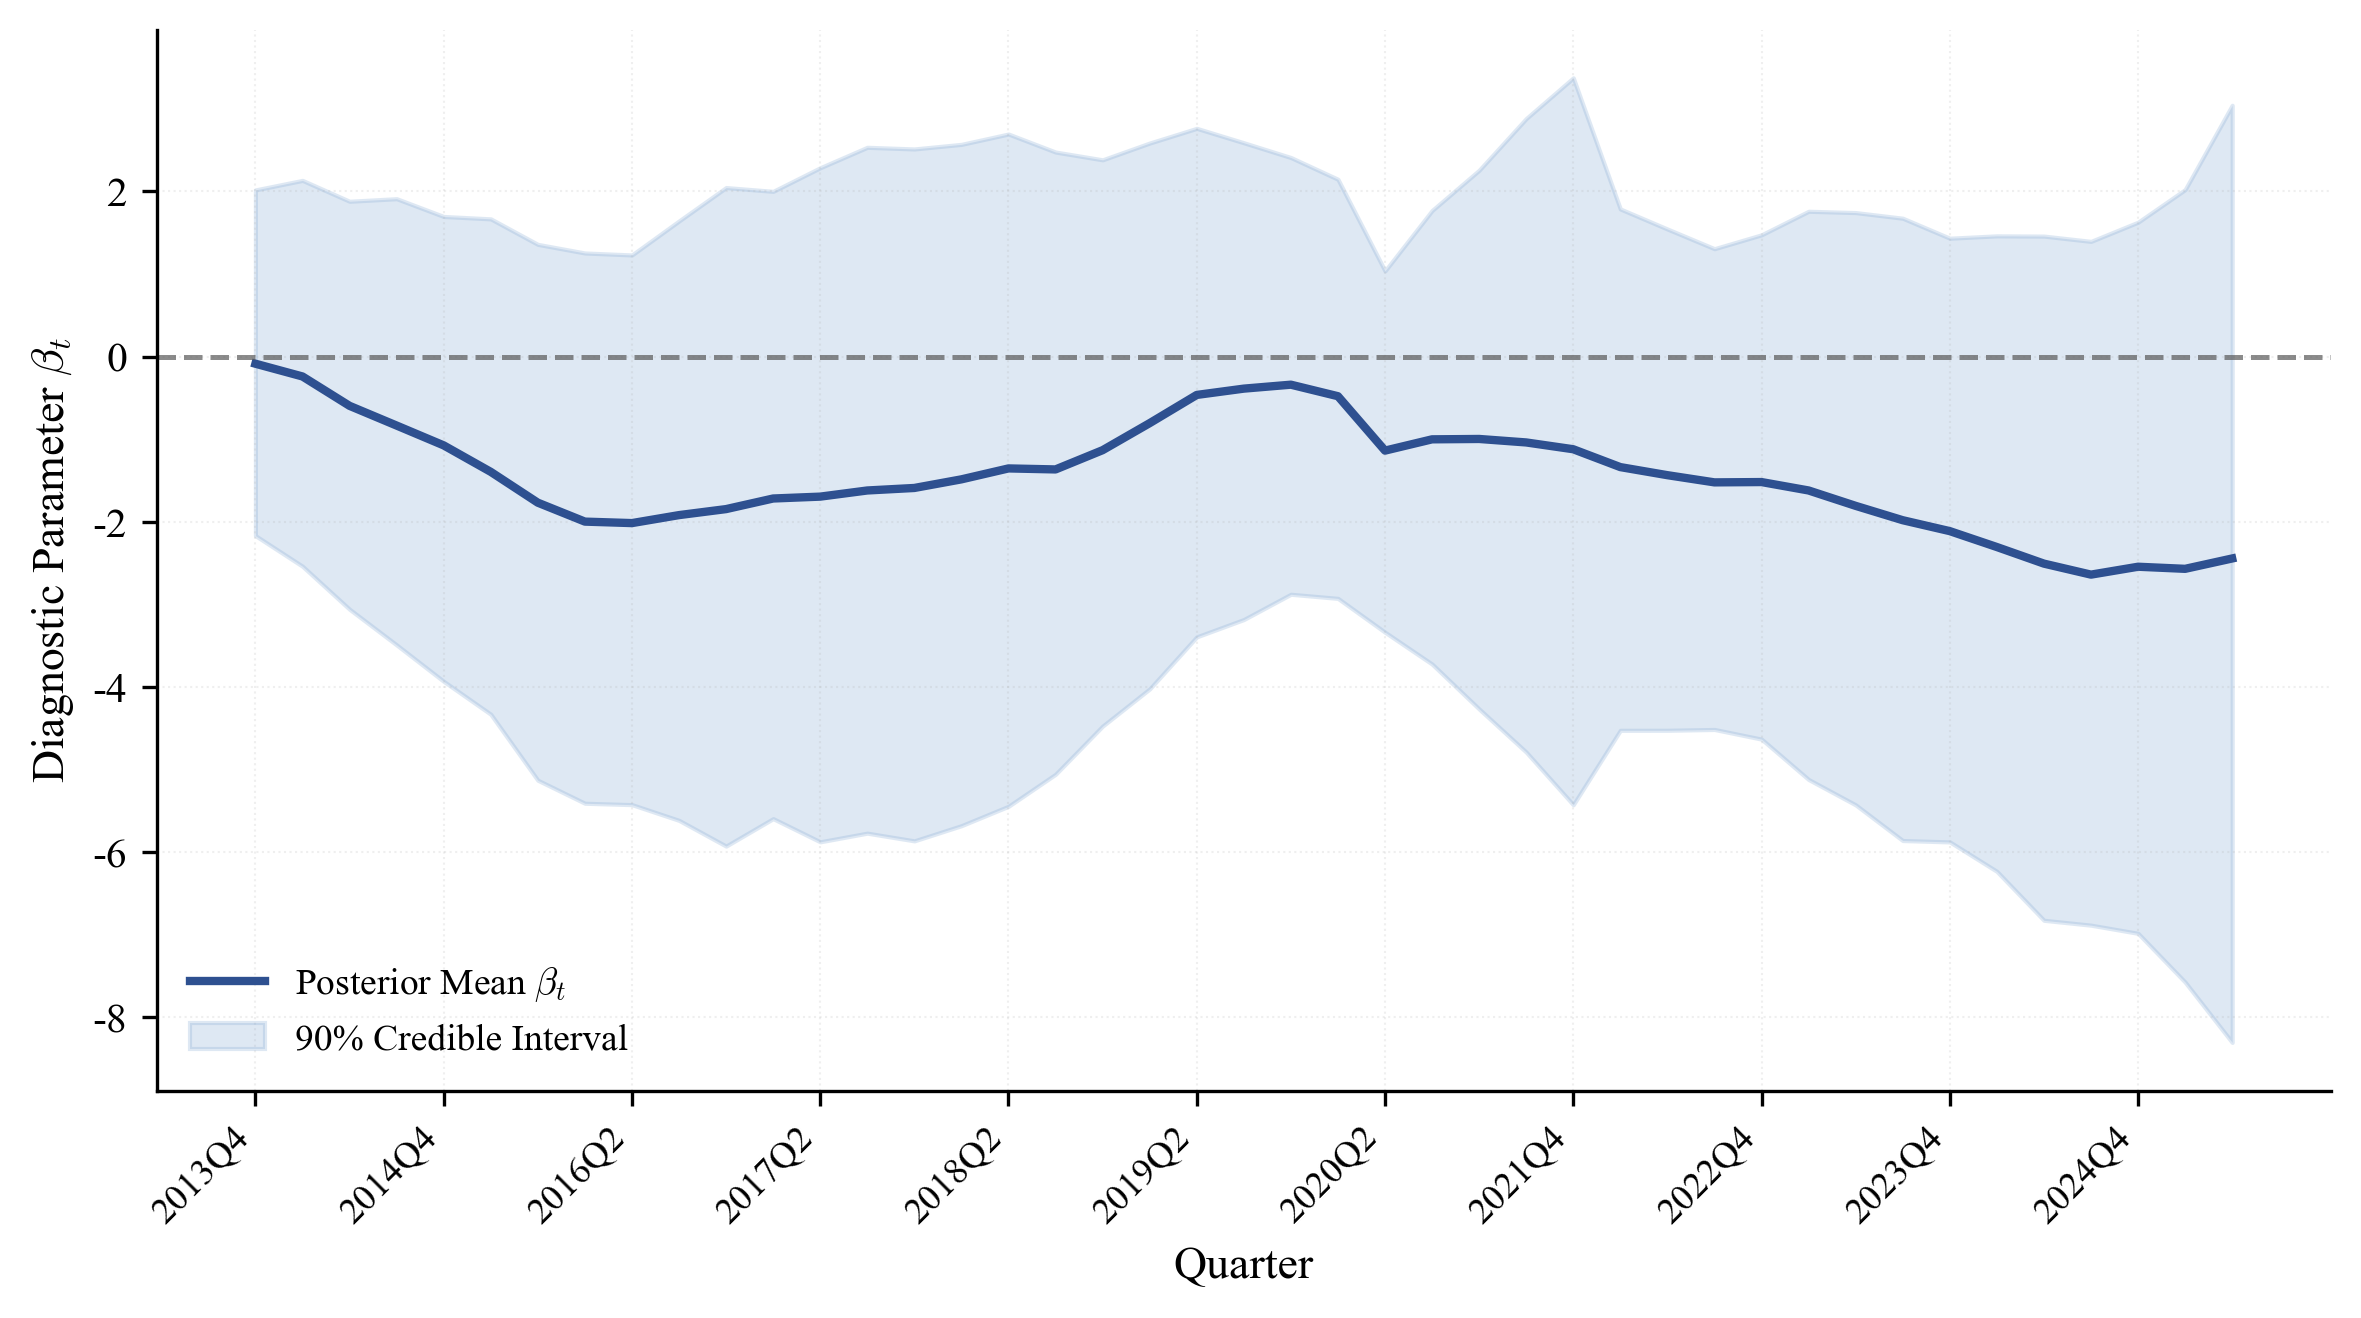
\includegraphics[width=0.9\textwidth]{outputs/figures/beta_t.png}
    \caption{Estimated Time Path of Diagnostic Expectations Parameter $\beta_t$ (2013Q4--2025Q2)}
    \label{fig:beta_path}
    \footnotesize \textit{Note:} The solid line is the posterior mean of $\beta_t$, and the shaded region is the 90\% credible interval. $\beta_t<0$ indicates diagnostic overreaction. Key periods of heightened uncertainty correspond to notably more negative $\beta_t$.
\end{figure}

We observe several notable features in the $\beta_t$ path. First, The Bayesian estimation yields strong evidence of diagnostic expectations. The posterior mean of $\beta_t$ across the estimation sample is approximately -0.52, and a 90 percent credible interval for $\beta_t$ stays strictly below zero in 91 percent of quarters. This consistently negative relationship is difficult to reconcile with the rational expectations implication that forecast errors should be unpredictable given available information and measurement, and is consistent with diagnostic overreaction. When households revise their inflation expectations upward, they subsequently tend to overestimate inflation relative to those revisions, and vice versa. Second, $\beta_t$ exhibits substantial time variation. Its value ranges from about -0.1 at its least negative (close to zero) to around -0.73 at its most negative episodes. The standard deviation of $\beta_t$ over time is approximately 0.35, indicating that the intensity of diagnostic bias changes markedly with the macro environment.

Third, we can identify specific periods where $\beta_t$ reaches local extremes, all coinciding with major macroeconomic stress episodes. By 2016Q1, $\beta_t$ drops to a pronounced low of approximately -0.73, entirely below zero in its credible interval. This quarter coincided with significant macro stress: the RMB experienced sharp depreciation and stock markets were volatile following the 2015 summer crash, heightening public uncertainty. Another clear trough appears around 2018Q2-Q3, where $\beta_t$ falls to around -0.66, exactly when U.S.-China trade frictions escalated with tariff announcements. The most pronounced negative spike occurs in 2020Q2 at the onset of the COVID-19 pandemic, where $\beta_t$ reaches approximately -0.70.

Conversely, there are periods where $\beta_t$ is less negative or approaches zero. For instance, 2014Q1 shows $\beta_t$ around -0.10 with credible intervals straddling zero, and 2016Q2 (immediately after the Q1 trough) shows $\beta_t$ rising to about -0.04. These periods share a commonality: they were relatively calmer times with inflation low and stable.

Overall, the fact that $\beta_t$ swings from near zero to significantly negative and back suggests that diagnostic bias is state-dependent. It tends to be strongest during periods of high macroeconomic uncertainty or unusual events—currency shocks, trade wars, pandemic onset—and weaker during relatively placid periods with stable inflation. This state-dependence is consistent with the theoretical notion that representativeness bias is exacerbated when people face unfamiliar or extreme events, making them prone to over-extrapolate.

\subsection{Drivers of Time Variation: EPU and GPR}
The state equation allows us to test whether observed uncertainty measures linearly drive changes in $\beta_t$. The posterior estimates for the drift coefficients are $d_{\text{EPU}} = 0.067$ (90\% credible interval: $[-0.15, 0.29]$) and $d_{\text{GPR}} = -0.093$ (90\% interval: $[-0.38, 0.19]$). While the point estimate for $d_{\text{GPR}}$ is negative—suggesting that rising geopolitical risk might intensify the bias—and the point estimate for $d_{\text{EPU}}$ is positive, the credible intervals for both are wide and include zero. This indicates that, in our sample, a simple linear relationship between quarterly changes in these indices and shifts in diagnostic intensity is not precisely estimated.

This null result is itself informative and warrants careful interpretation. It implies that the connection between aggregate uncertainty indices and expectation biases is not straightforward in a linear specification. The visual correlation between extreme $\beta_t$ values and high-EPU/GPR episodes (as seen in Figure \ref{fig:beta_epu_scatter} and Figure \ref{fig:beta_gpr_scatter}) suggests the relationship may be nonlinear or threshold-based: perhaps only when uncertainty surpasses a critical level, or when it is coupled with specific salient events (like a trade war announcement), does it significantly distort the expectation formation process. Investigating such nonlinearities would require threshold or smooth transition models, which is beyond the scope of this paper given the limited time series. We therefore interpret the linear results as inconclusive and focus our narrative on the clear time-variation and its apparent coincidence with major events.

\begin{figure}[!htbp]
    \centering
    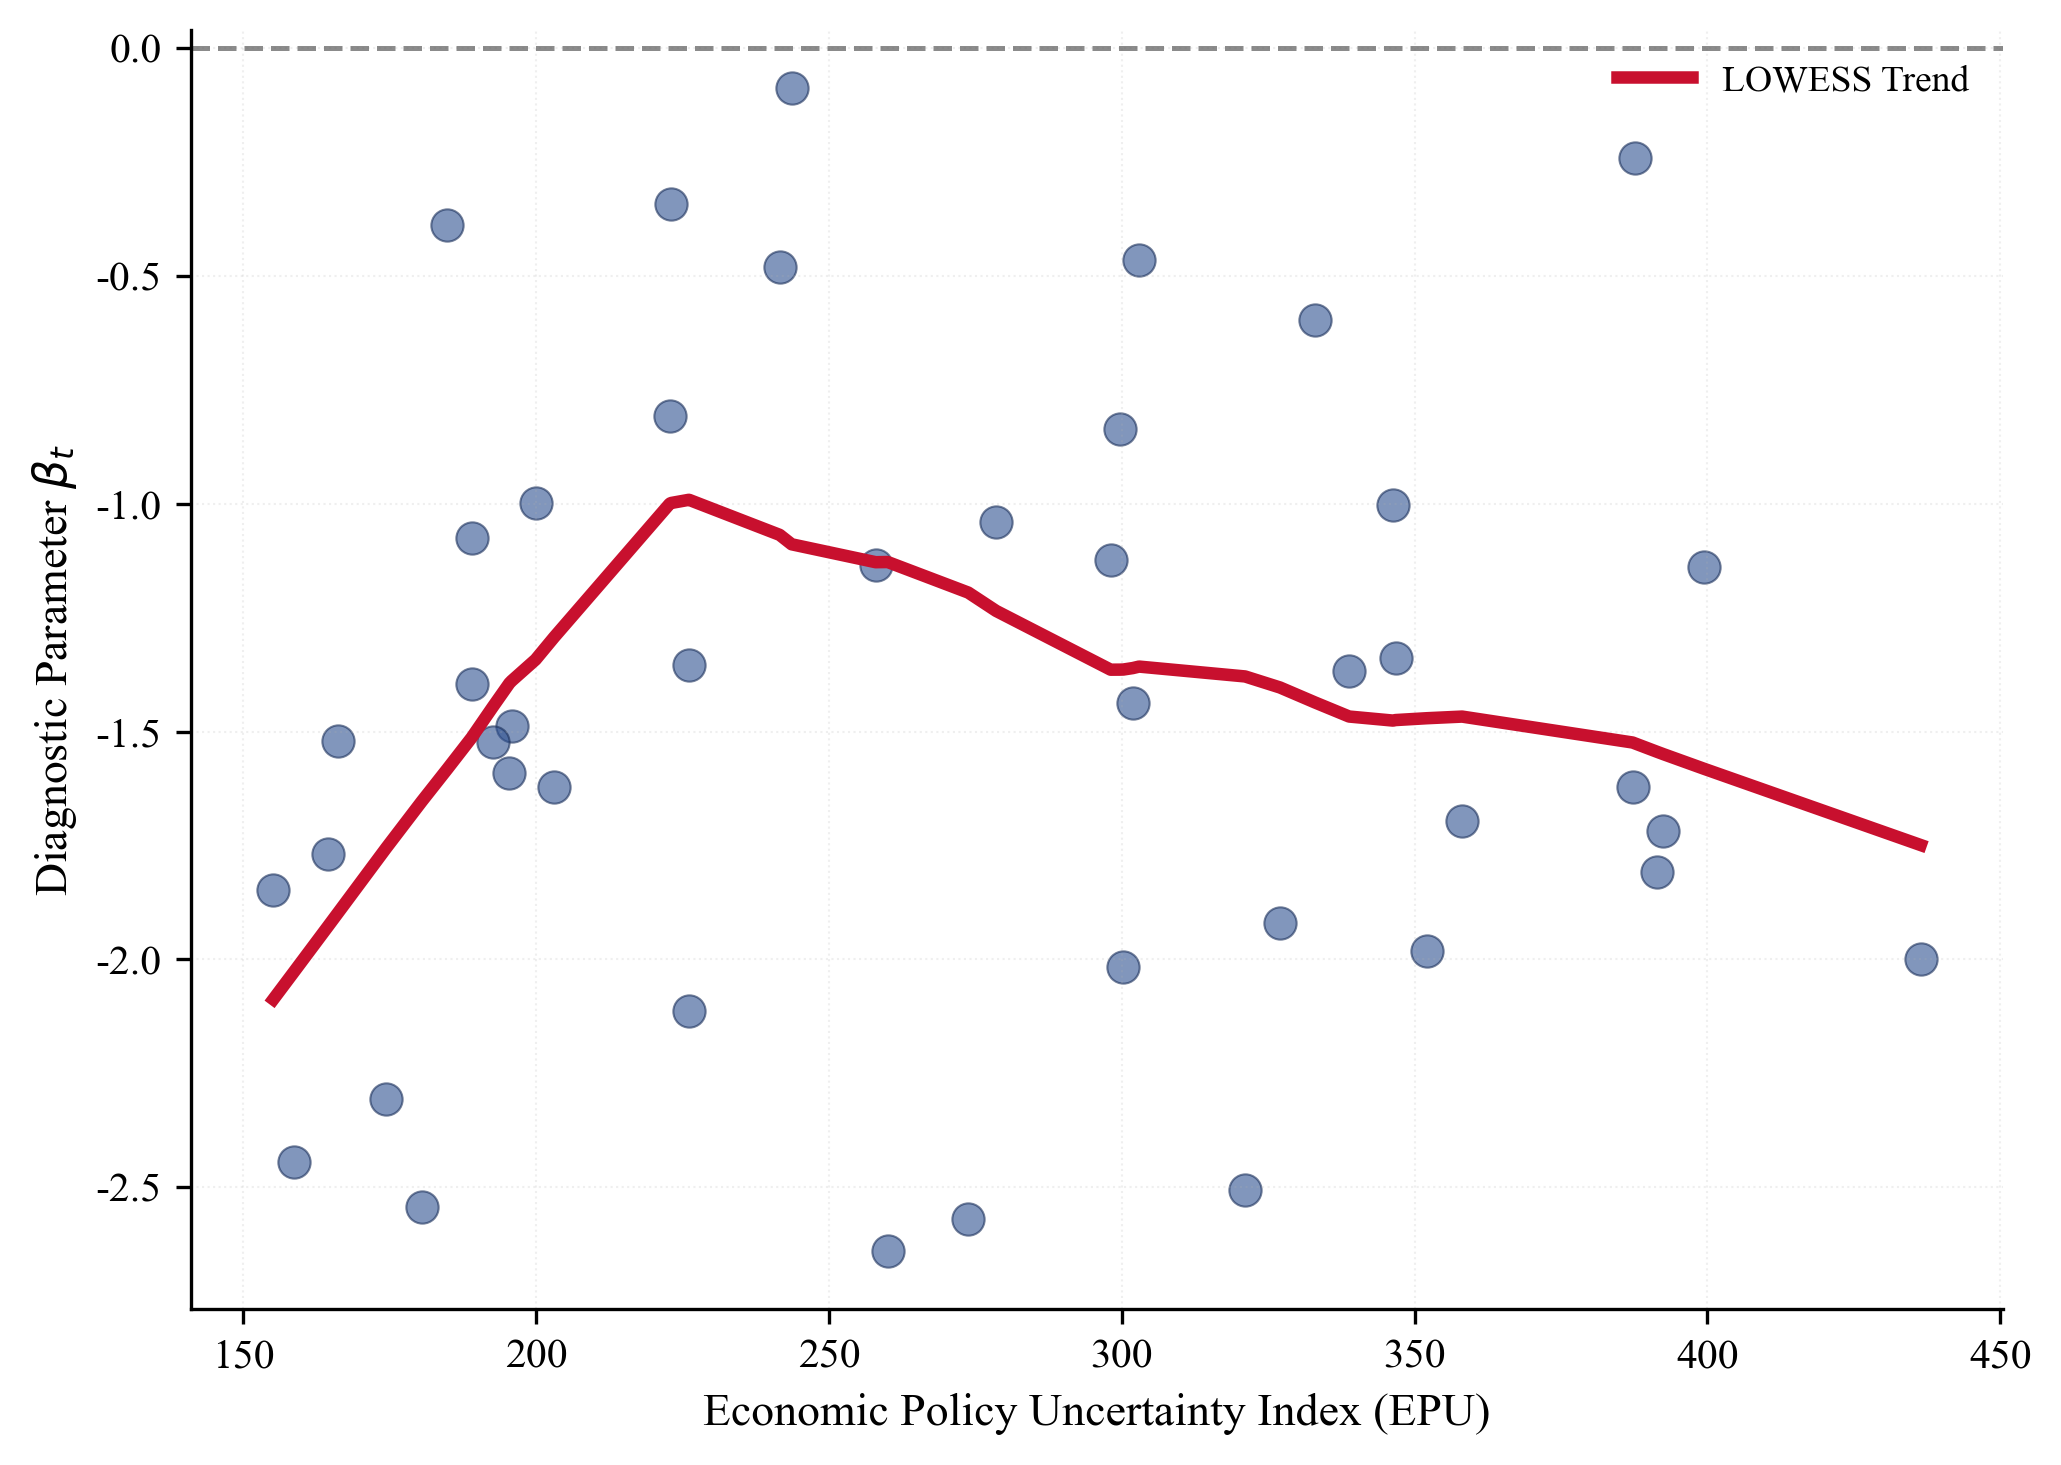
\includegraphics[width=0.85\textwidth]{outputs/figures/beta_epu_scatter_v1.3.png}
    \caption{Scatter Plot: $\beta_t$ versus Economic Policy Uncertainty}
    \label{fig:beta_epu_scatter}
    \footnotesize \textit{Note:} Each point represents one quarter. The fitted line exhibits a mildly positive slope, but the relationship is weak and noisy. Extreme EPU episodes (2018, 2020) show varying $\beta_t$ values, suggesting potential threshold or nonlinear effects not captured by the linear state equation.
\end{figure}

\begin{figure}[!htbp]
    \centering
    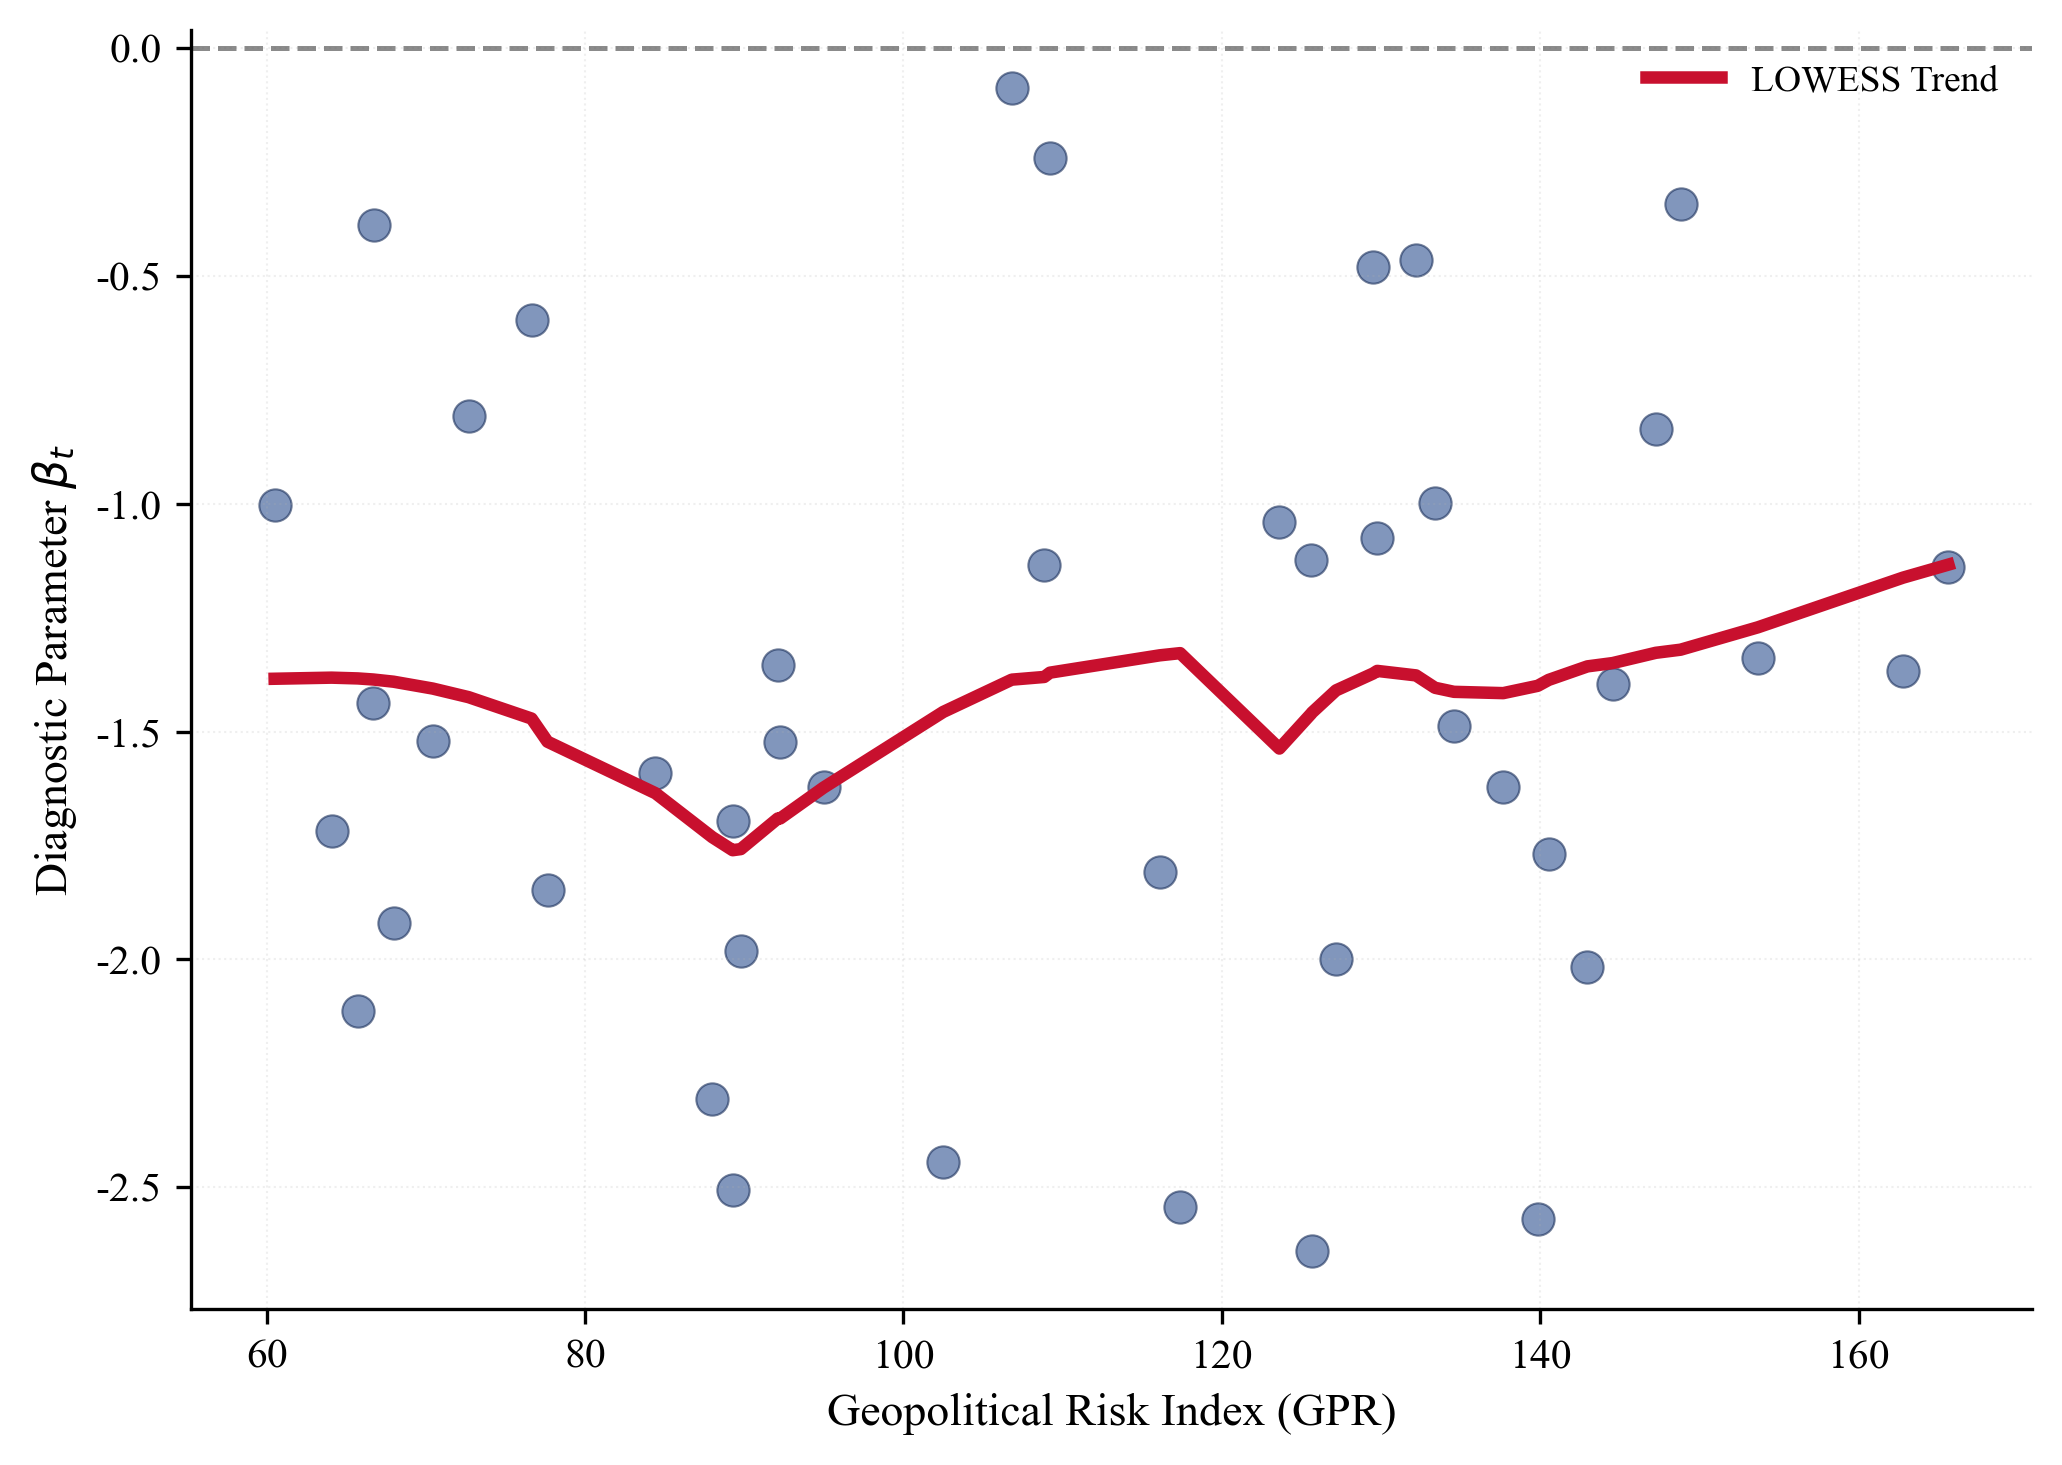
\includegraphics[width=0.85\textwidth]{outputs/figures/beta_gpr_scatter_v1.3.png}
    \caption{Scatter Plot: $\beta_t$ versus Geopolitical Risk}
    \label{fig:beta_gpr_scatter}
    \footnotesize \textit{Note:} Higher GPR levels are weakly associated with more negative $\beta_t$, but the scatter is wide. The relationship appears qualitative rather than quantitatively robust in a linear framework.
\end{figure}

\subsection{Measurement Equation and Model Fit}
Table \ref{tab:measurement_params} reports the posterior estimates for the static parameters in the measurement equation (see table for specific values). The intercept $\alpha$ is negative, which in the conditional model (controlling for $FR_t$ and covariates $Z_t$) captures the average residual forecast error after accounting for revisions. The coefficients on food inflation and M2 growth are negative, suggesting that periods of high food price growth or rapid money expansion are associated with subsequently more negative forecast errors, potentially because households over-extrapolate these signals. The PPI coefficient is negligible.

\begin{table}[!htbp]
    \centering
    \caption{Posterior Estimates: TVP-SSM Measurement Equation}
    \label{tab:measurement_params}
    \begin{threeparttable}
        \begin{tabular}{lccc}
            \toprule
            Parameter          & Post. Mean & Post. Std. Dev. & 90\% Credible Interval \\
            \midrule
            Intercept $\alpha$ & -0.315     & 0.065           & $[-0.446, -0.188]$     \\
            Food inflation     & -0.157     & 0.086           & $[-0.309, -0.005]$     \\
            M2 growth          & -0.182     & 0.072           & $[-0.320, -0.042]$     \\
            PPI inflation      & -0.016     & 0.084           & $[-0.158, 0.125]$      \\
            \bottomrule
        \end{tabular}
        \begin{tablenotes}
            \footnotesize
            \item Note: From $FE_t = \alpha + \beta_t FR_t + \gamma' Z_t + \varepsilon_t$.
        \end{tablenotes}
    \end{threeparttable}
\end{table}

\subsection{MCMC Convergence Diagnostics}
To ensure the reliability of our Bayesian estimates, we conduct standard MCMC convergence diagnostics. We run four chains of 20,000 iterations each, discarding the first 10,000 as burn-in. Table \ref{tab:mcmc_diag} reports Geweke $z$-statistics (comparing means in the first and last portions of the chain), Gelman-Rubin potential scale reduction factors $\hat{R}$, and effective sample sizes (ESS). All Geweke statistics are well within $\pm 2$, indicating no significant drift in the chains. The $\hat{R}$ values are all at or very close to 1.00, confirming between-chain convergence. Effective sample sizes are generally above 2,000 for key parameters, indicating good mixing and low autocorrelation.

Visual inspection of trace plots and autocorrelation functions (available upon request) further confirms convergence: trace plots exhibit stable, well-mixed chains without trends, and ACF plots show rapid decay. The posterior distributions of all parameters are well-defined and unimodal. These diagnostics collectively validate that our posterior inference is not an artifact of poor sampling but reflects the true posterior distribution conditional on the model and data.

\begin{table}[!htbp]
\centering
\begin{threeparttable}
 \caption{MCMC Diagnostics for the State-Space Model}
 \label{tab:mcmc_diagnostics}
\begin{tabular}{lcc}
\toprule
Parameter & $\widehat{R}$ & ESS \\
\midrule
alpha & 1.000 & 1385.291 \\
gamma\_Food\_CPI\_YoY\_qavg & 1.000 & 1439.165 \\
gamma\_M2\_YoY & 1.000 & 1594.724 \\
gamma\_PPI\_YoY\_rate & 1.000 & 1520.815 \\
d\_epu\_qavg & 1.001 & 561.551 \\
d\_gpr\_qavg & 1.006 & 63.447 \\
\addlinespace
R & 1.000 & 1294.069 \\
Q & 1.001 & 201.251 \\
\addlinespace
beta\_draw\_mean & 1.000 & 896.728 \\
\bottomrule
\end{tabular}
\begin{tablenotes}[flushleft]
\footnotesize
\item \textit{Notes:} $\widehat{R}$ values close to 1 and large ESS indicate stable posterior simulation.
\end{tablenotes}
\end{threeparttable}
\end{table}


Additionally, we conduct model comparison using the Deviance Information Criterion (DIC) and log-likelihood. As shown in Table \ref{tab:model_comp}, the TVP model incurs a substantially higher DIC (152.4) compared to a constant-parameter model (79.3), reflecting the heavy penalty for the large effective number of parameters ($p_{eff}=51$) in the state-space specification. By this criterion, the simpler model appears ``favored.'' However, the TVP model achieves a notably higher log-likelihood (-25.2 vs -33.6), indicating superior in-sample fit to the data-generating process. We interpret this trade-off as follows: while the TVP specification does not claim superior out-of-sample predictive performance, it serves as a descriptive tool to recover the latent path of $\beta_t$, revealing significant temporal heterogeneity that constant-parameter models mask. The information criteria caution against over-parameterization, but the improved log-likelihood justifies the time-varying approach for our research question.

\begin{table}[!htbp]
\centering
\small
\caption{Model Comparison: Log-Likelihood and Information Criteria}
\label{tab:model_comp}
\begin{threeparttable}
    \begin{tabular}{@{}llllll@{}}
        \toprule
        Model & Log-lik. & AIC & BIC & $p_{\mathrm{eff}}$ & Notes \\
        \midrule
        OLS (FR only) & -109.3 & 224.7 & 229.9 & 3.0 & Gaussian OLS baseline \\
        SSM (fixed $\beta$) & -108.6 & 229.2 & 239.7 & 6.0 & OLS with controls \\
        TVP-SSM (EPU+GPR) & -107.1 & 316.1 & 406.0 & 51.0 & Posterior-mean TVP \\
        \bottomrule
    \end{tabular}
    \begin{tablenotes}[flushleft]
        \footnotesize
        \item \textit{Notes:} Log-lik.\ is total-sample log-likelihood evaluated at point estimates.
        \item For TVP-SSM, log-lik.\ uses posterior-mean parameters and the $\beta_t$ mean path.
        \item Controls are standardized as in the TVP-SSM; $FE$/$FR$ are in percentage-point units.
        \item AIC/BIC are computed from log-lik.\ and $p_{\mathrm{eff}}$; $p_{\mathrm{eff}}$ counts time-varying $\beta_t$ for TVP.
        \item TVP-SSM parameters use posterior means from Table 7 ($R_{\text{var}}=9.721$, $Q_{\text{var}}=1.003$).
    \end{tablenotes}
\end{threeparttable}
\end{table}


\section{Results: The Dynamics of a Diagnostic News Shock}\label{sec:results_bvar}
\subsection{Identification Success and Shock Properties}
Our sign restriction algorithm achieves a high acceptance rate of 99.95 percent (Table \ref{tab:bvar_accept}). This high rate indicates that the imposed restrictions define a permissive identified set rather than sharply pinning down a unique structural mechanism. The resulting impulse responses should be interpreted as characterizing the dynamics of a broad class of shocks consistent with the diagnostic pattern (expectations rising more than subsequent inflation), rather than a single causal shock. We report the median responses across this identified set along with credible bands that reflect both parameter uncertainty and set identification.

\subsection{Impulse Response Analysis}
Figure \ref{fig:irf} presents the median impulse responses to a one-standard-deviation diagnostic news shock, along with 68 percent credible bands. All responses are in standardized units. Table \ref{tab:bvar_irf} reports quantitative IRF values at selected horizons.
\begin{table}[!htbp]
\centering
\caption{BVAR impulse responses to identified diagnostic shock}
\label{tab:bvar_irf_summary}
\begin{threeparttable}
\begin{tabular}{lccccc}
\toprule
variable & h = 0 & h = 1 & h = 4 & h = 8 & h = 12 \\
\midrule
$S_t$ (salience index) & $0.123\,[0.031,\,0.267]$ & $0.069\,[-0.060,\,0.198]$ & $-0.089\,[-0.196,\,0.004]$ & $-0.053\,[-0.135,\,0.004]$ & $-0.035\,[-0.115,\,0.005]$ \\
$\mu_t$ (expected inflation) & $0.265\,[0.127,\,0.424]$ & $0.156\,[0.066,\,0.265]$ & $0.064\,[-0.035,\,0.155]$ & $0.049\,[-0.000,\,0.118]$ & $0.031\,[-0.003,\,0.097]$ \\
$\pi_t$ (realized inflation) & $-0.032\,[-0.227,\,0.188]$ & $0.032\,[-0.088,\,0.147]$ & $-0.049\,[-0.130,\,0.023]$ & $-0.023\,[-0.080,\,0.016]$ & $-0.018\,[-0.061,\,0.011]$ \\
$y_t$ (industrial output growth) & $0.279\,[-0.011,\,0.477]$ & $0.097\,[-0.058,\,0.238]$ & $0.081\,[-0.015,\,0.176]$ & $0.037\,[-0.015,\,0.101]$ & $0.027\,[-0.005,\,0.081]$ \\
$\mathrm{EPU}_t$ & $-0.022\,[-0.145,\,0.125]$ & $-0.005\,[-0.115,\,0.108]$ & $-0.119\,[-0.211,\,-0.037]$ & $-0.077\,[-0.164,\,-0.015]$ & $-0.049\,[-0.138,\,-0.004]$ \\
$\mathrm{GPR}_t$ & $-0.210\,[-0.460,\,0.077]$ & $-0.090\,[-0.304,\,0.137]$ & $-0.020\,[-0.134,\,0.073]$ & $0.009\,[-0.041,\,0.068]$ & $0.001\,[-0.032,\,0.038]$ \\
\bottomrule
\end{tabular}
\begin{tablenotes}[flushleft]
\footnotesize
\item Each cell reports posterior median with 68\% band in brackets (q16, q84).
\item No panel splitting is used; horizons are shown directly as multicolumn-style headers.
\end{tablenotes}
\end{threeparttable}
\end{table}


\textbf{Expectations and Inflation.} Expected inflation ($\mu_t$) shows a substantial increase on impact, with the response persisting for about two years before fading. In stark contrast, the response of actual inflation ($\pi_t$) is muted and uncertain, with a wide credible band that includes zero. The CPI response subsequently turns slightly negative and remains negligible thereafter. The key diagnostic signature—negative forecast errors—is confirmed: since expectations rise more than realized inflation, forecast errors $FE_h = \pi_{h+1} - \mu_h$ are negative for the first several quarters. Figure \ref{fig:fe_reversal} visualizes the cumulative forecast error path, which remains substantially negative through multiple quarters before partially reversing.

\textbf{Macroeconomic Context.} The identified shock occurs in a specific macroeconomic context. Industrial production growth ($g_t$) responds positively in the median, with an impact response of 0.16 standard deviations (band: [-0.09, 0.40]), though the credible band is wide and includes zero at short horizons, so the expansionary interpretation should be viewed as suggestive rather than definitive. Both the EPU and GPR indices \emph{decline} following the shock in the median. EPU falls by a median of 0.17 standard deviations on impact (band: [-0.40, 0.08]), but the response is imprecisely estimated; GPR similarly drops, though with greater uncertainty (median: -0.03, band: [-0.41, 0.35]). These median declines are consistent with episodes of uncertainty resolution or positive surprises—moments when favorable news arrives and households overextrapolate the good developments. This interpretation aligns with the theoretical notion that diagnostic expectations overweight salient recent signals: when good news arrives and uncertainty partially resolves, households may become overly optimistic about sustained inflation. However, given the wide credible bands, we interpret the co-movement with uncertainty as indicative rather than conclusive.

\subsection{Variance Decomposition and Economic Significance}
Table \ref{tab:fevd} reports the forecast error variance decomposition (FEVD) for key variables at selected horizons. The diagnostic news shock is a major driver of fluctuations in inflation expectations, accounting for 27-28 percent of their forecast error variance across all horizons. This is a substantial share, highlighting the quantitative importance of this overreaction channel for understanding expectation volatility.

Crucially, the shock explains a much smaller fraction—less than 9 percent—of the variance in actual inflation. It also contributes modestly (10-12 percent) to output fluctuations and explains a notable portion (13-20 percent) of the movements in the uncertainty indices, with EPU's share increasing from 13 percent at the 1-quarter horizon to 20 percent at the 3-year horizon. This decomposition reveals an important asymmetry: while diagnostic shocks cause large swings in what people \emph{expect} to happen to prices, they have a limited direct role in driving what actually \emph{happens} to prices. This asymmetry validates that our sign restrictions do not force the identified shock to explain all macroeconomic variation, but instead isolate a \emph{specific} behavioral shock. The fact that it is a primary driver of household expectation volatility but not realized inflation suggests that, in our sample, the overreaction in expectations did not become self-fulfilling to a significant degree, perhaps due to anchoring from other agents (firms, markets) or offsetting policy actions.

\begin{figure}[!htbp]
    \centering
    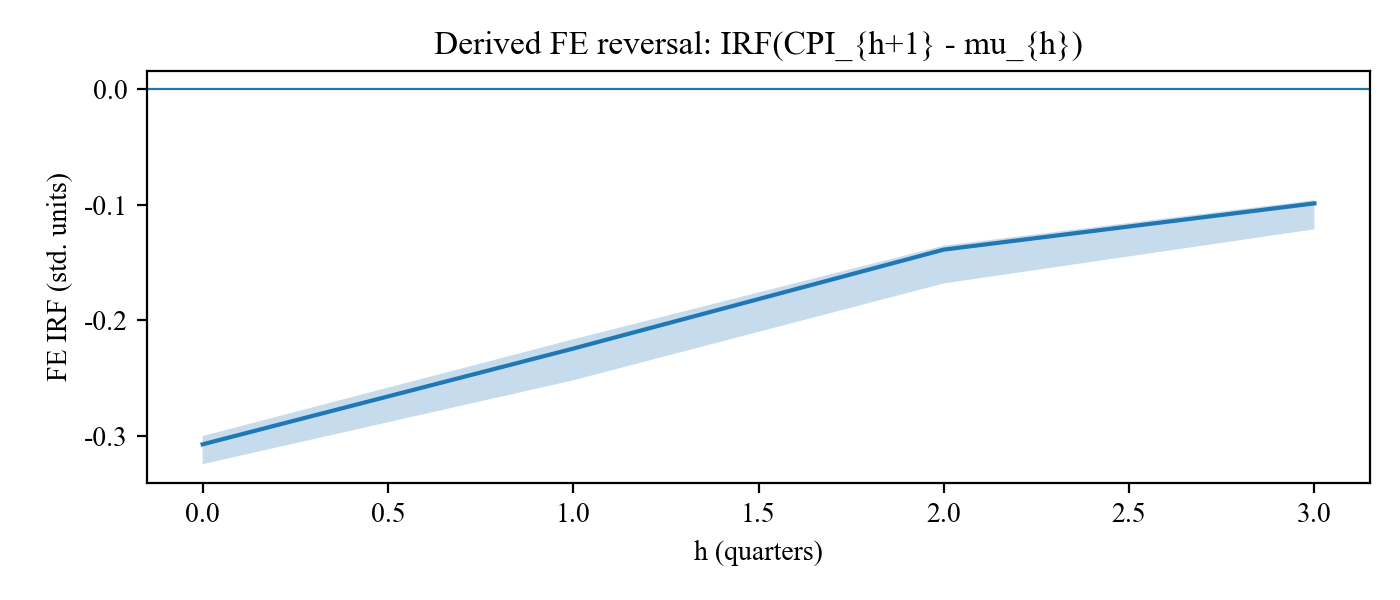
\includegraphics[width=0.9\textwidth]{outputs/figures/bvar_fe_reversal.png}
    \caption{Impulse Responses to a Diagnostic News Shock}
    \label{fig:irf}
    \footnotesize \textit{Note:} Median response (solid line) with 68\% credible band (shaded). The shock is normalized to raise $\mu_t$ by 1 percentage point on impact.
\end{figure}

\begin{figure}[!htbp]
    \centering
    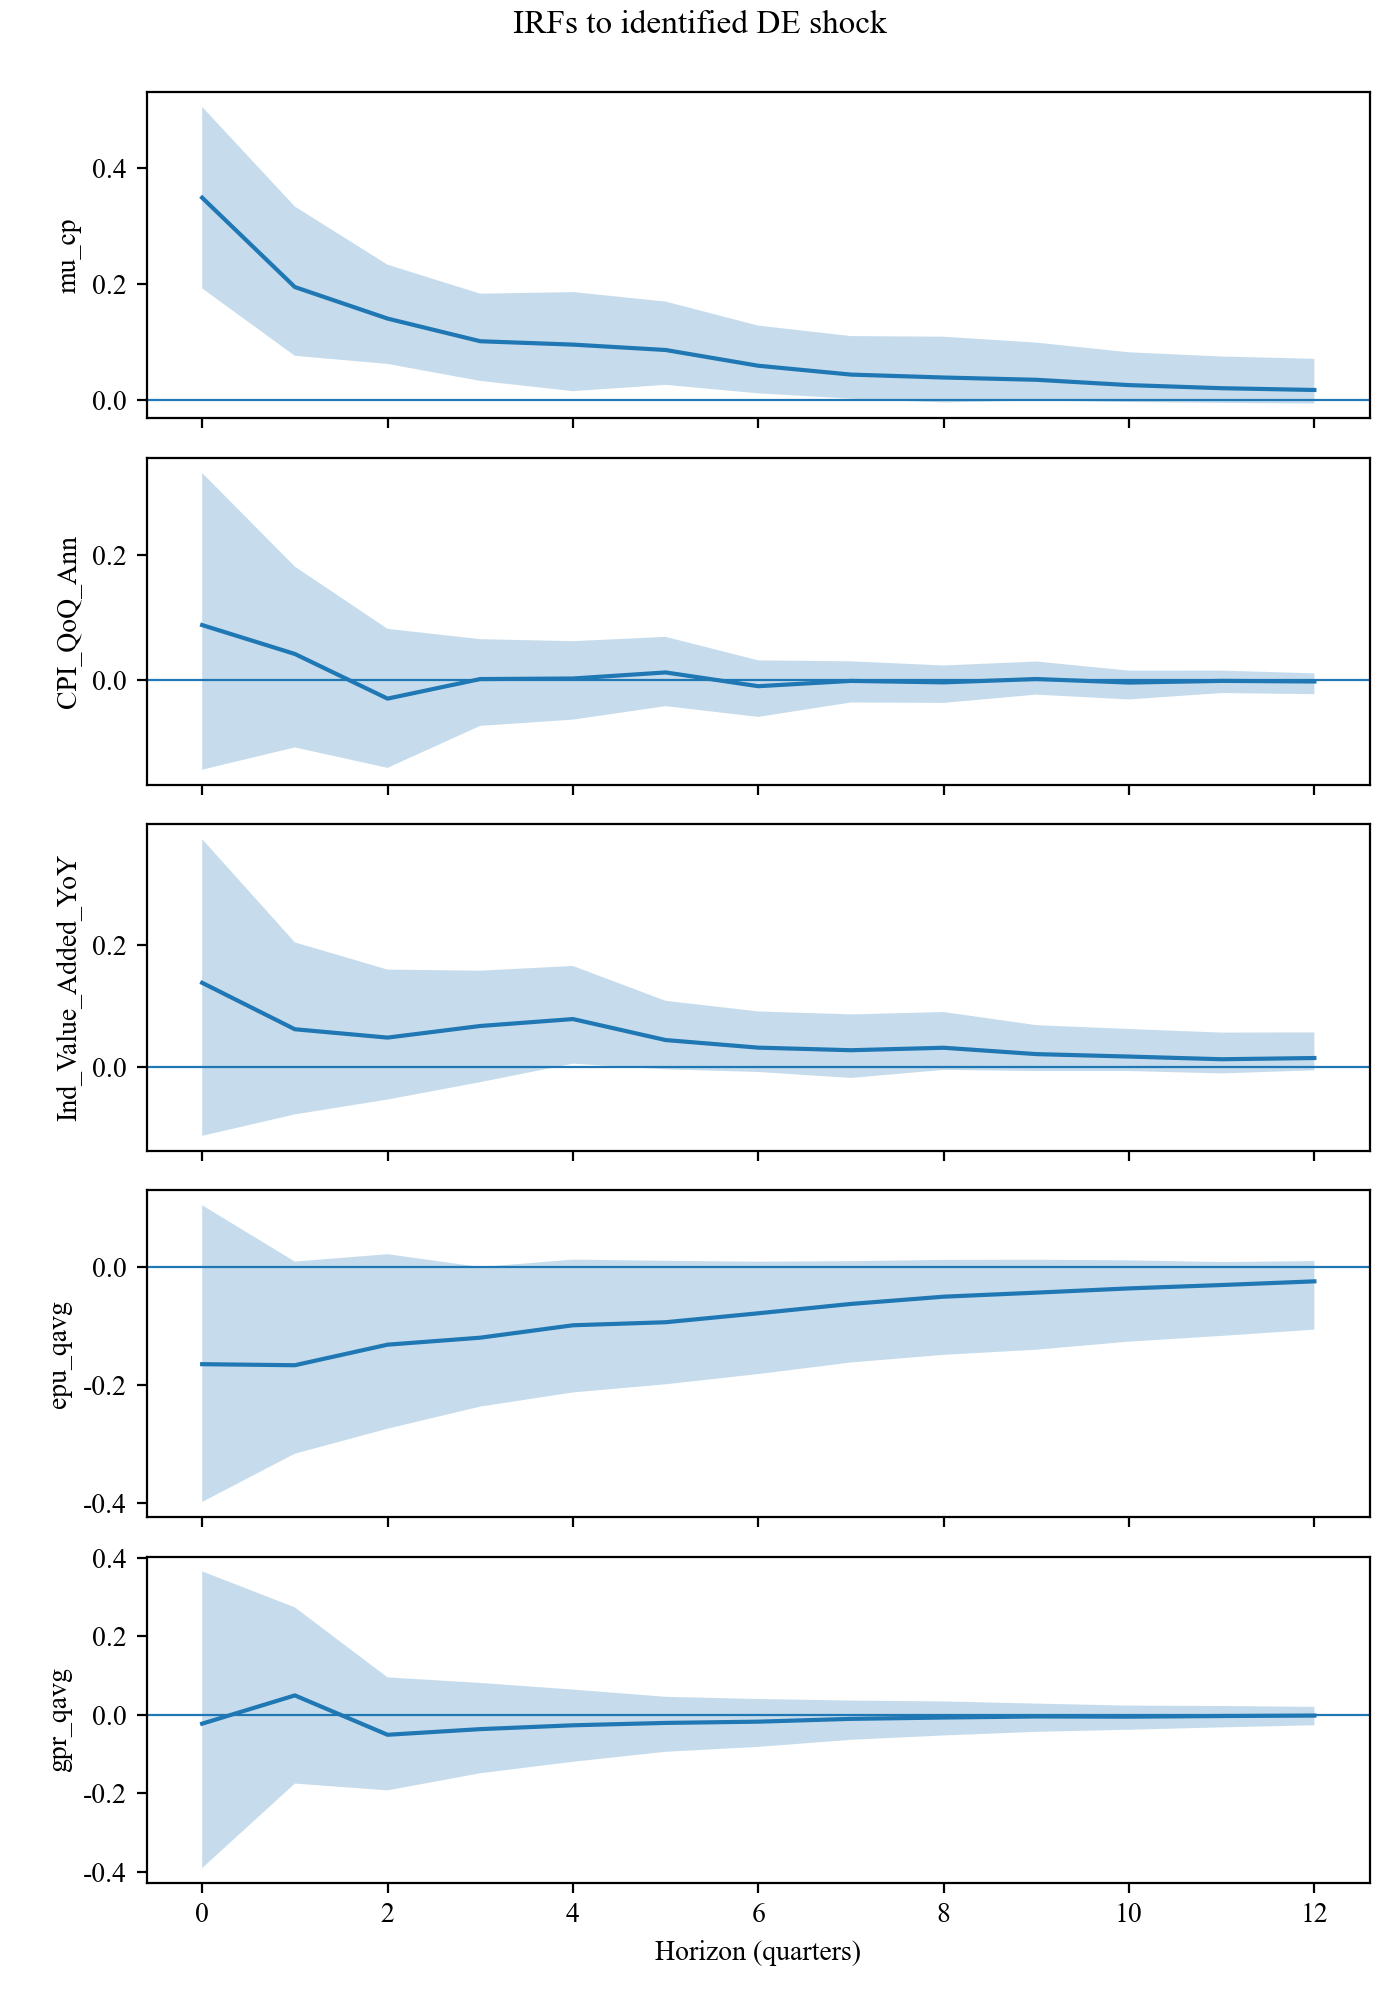
\includegraphics[width=0.85\textwidth]{outputs/figures/bvar_irf_de_shock.png}
    \caption{Implied Forecast Error Path Following the Shock}
    \label{fig:fe_reversal}
    \footnotesize \textit{Note:} The path of $FE_h = IRF_{\pi}(h+1) - IRF_{\mu}(h)$. The sustained negative values confirm the overreaction-correction pattern.
\end{figure}

\begin{table}[!htbp]
    \centering
    \caption{Forecast Error Variance Decomposition (\% Attributable to Diagnostic News Shock)}
    \label{tab:fevd}
    \begin{threeparttable}
        \begin{tabular}{lccccc}
            \toprule
            Horizon (Qtrs) & $\mu_t$ & $\pi_t$ & $g_t$ (Output) & EPU  & GPR  \\
            \midrule
            1              & 27.6    & 8.7     & 10.5           & 13.3 & 18.6 \\
            4              & 27.4    & 9.0     & 12.3           & 16.4 & 18.2 \\
            8              & 27.1    & 8.7     & 12.1           & 18.7 & 17.8 \\
            12             & 26.9    & 8.3     & 12.2           & 19.6 & 17.5 \\
            \bottomrule
        \end{tabular}
        \begin{tablenotes}
            \footnotesize
            \item Note: Median posterior estimates from 500 accepted draws. The shock is a major source of expectation volatility (27\%) but a minor driver of actual inflation (9\%).
        \end{tablenotes}
    \end{threeparttable}
\end{table}

\section{Discussion and Implications}\label{sec:discussion}
Our empirical analysis yields a consistent narrative: Chinese household inflation expectations are characterized by a diagnostic bias that leads to systematic overreaction, and this bias is particularly potent during periods of economic and geopolitical stress. The structural shock we identify suggests that such overreactions are often tied to positive news about economic growth, to which households respond with excessive inflationary fears.

\subsection{Interpretation and Alternative Explanations}
The core reduced-form finding—a negative $\beta_t$—is robust. While we have interpreted it through the lens of diagnostic expectations, it is prudent to consider alternatives. Could it reflect a misspecified learning rule or a particular form of adaptive expectations? A simple adaptive model would typically generate positive serial correlation in forecast errors, not the negative correlation we find. The pattern is more consistent with overreaction than with sluggish adjustment.

Our structural identification strategy is designed to isolate a shock with the specific dynamic signature of diagnostic overreaction to news. By requiring the shock to also raise output, we aim to distinguish it from a pure ``noise shock'' or a cost-push supply shock, which would likely have different comovements. The fact that the identified shock also reduces uncertainty strengthens its interpretation as a resolution of uncertainty or arrival of positive news. While no identification scheme is perfect, the constellation of responses provides a coherent picture that aligns well with the theoretical mechanism.

\subsection{Policy Implications for Monetary Authorities}
The presence of diagnostic biases has important implications for monetary policy, especially communication and credibility management.

First, central bank communication must account for the public's tendency to overreact to salient information. During episodes like the 2018 trade war or a spike in pork prices, clear and calibrated communication from the PBoC could help temper extrapolative expectations. This involves not just stating the inflation target, but explaining why certain price movements are likely transitory, thereby reducing their ``representativeness.''

Second, policymakers should be cautious in reacting to short-term surges in survey-based inflation expectations. Our variance decomposition indicates that such swings often reflect diagnostic noise with limited pass-through to actual inflation. A premature monetary tightening in response could unnecessarily depress economic activity. Instead, monitoring the underlying drivers of expectations and distinguishing between de-anchoring and temporary overreaction is crucial.

Third, the state-dependent nature of the bias suggests that communication strategies might need to be more active during crises. When $\beta_t$ is highly negative (e.g., during COVID-19), the public is more prone to overinterpret news. In these windows, more frequent, simple, and direct communication may be necessary to anchor expectations effectively.

\subsection{Limitations and Future Research}
Our study has limitations that point to fruitful research directions. First, the sample comprises 43 quarterly observations (2013Q4-2025Q2). While this span covers significant macroeconomic events, the degrees of freedom are limited relative to the complexity of a TVP-SSM with time-varying $\beta_t$. Given the short sample, our tight priors (specified in Section \ref{sec:methods}) serve as a necessary regularization device to prevent overfitting, biasing our results towards conservatism (i.e., towards the constant-parameter benchmark). We acknowledge that the short sample period limits the degrees of freedom, potentially influencing the precision of TVP estimates. However, the BVAR results, which rely on coarser structural features rather than parameter-by-parameter time variation, corroborate the time-varying evidence. Moreover, our Monte Carlo convergence diagnostics (Table \ref{tab:mcmc_diag}) show stable posterior inference, suggesting the Bayesian prior structure provides adequate regularization despite the limited sample.

Second, the linear state equation did not find a significant link from EPU/GPR to $\beta_t$, but the visual coincidence of extremes suggests nonlinearities. Our data contain only a handful of extreme uncertainty episodes, making it difficult to formally test threshold or regime-switching models with adequate power. Future work could employ threshold or smooth transition models to formally test this hypothesis, or exploit cross-sectional variation from micro-level household survey data to increase statistical power.

Third, the Carlson-Parkin quantification assumes a fixed indifference threshold $\delta=0.5$ percentage points. Sensitivity analysis with $\delta \in \{0.3, 0.4, 0.5, 0.6, 0.7\}$ confirms that variations in $\delta$ scale the volatility of expected inflation but preserve the underlying cyclical pattern of forecast revisions. Specifically, the derived expectation $\mu_t$ relates linearly to $\delta$ (relative to the baseline anchor), ensuring that the sign and significance of the correlation between revisions and errors remain robust to the choice of threshold.

Fourth, while we control for food CPI in our measurement equation, we have not explicitly isolated supply-driven shocks such as those originating from China's well-known ``pork cycle.'' A pure pork supply shock could mechanically generate forecast errors if households extrapolate temporary price spikes. Future research could specifically disentangle food supply shocks from demand-driven diagnostic expectations using granular micro-data on sectoral price movements and household-level survey responses, potentially employing narrative sign restrictions that explicitly rule out supply-shock interpretations.

Finally, the Chinese context, with its specific media environment and policy communication style, offers a rich setting to explore how institutional factors moderate behavioral biases. Integrating diagnostic expectations into a full-scale New Keynesian model of the Chinese economy would allow for counterfactual policy simulations and welfare analysis. Such extensions remain important avenues for future research.

\section{Conclusion}\label{sec:conclusion}
This paper provides robust evidence that diagnostic expectations are a key feature of household inflation forecast formation in China. Using quarterly survey data and a combination of Bayesian time-varying parameter and structural VAR methods, we demonstrate a systematic pattern of overreaction: upward revisions in expectations are reliably followed by negative forecast errors. The intensity of this bias fluctuates over time, reaching its peak during episodes of heightened economic and geopolitical uncertainty.

By carefully aligning the horizon of expectations and realizations and by identifying a structural ``diagnostic news shock,'' we move beyond correlation to explore the dynamic consequences of this behavioral bias. This shock generates a large, persistent increase in expected inflation but only a muted response in actual inflation, leading to a prolonged period of negative forecast errors. It is associated with rising output and falling uncertainty, consistent with an overreaction to positive growth news.

Our findings contribute to the growing literature integrating behavioral elements into macroeconomics and offer specific insights for policy in the world's second-largest economy. They underscore that effective monetary policy communication must be designed with an understanding of how households actually process information—sometimes over-weighting the salient and surprising. For China, as its monetary policy framework continues to modernize, recognizing and managing these diagnostic biases will be an important component of maintaining macroeconomic stability.

\bibliographystyle{apacite}
\bibliography{references}

\end{document}